% Created 2021-04-13 Tue 20:45
% Intended LaTeX compiler: pdflatex
\documentclass[presentation,bigger,aspectratio=169]{beamer}
\usepackage[utf8]{inputenc}
\usepackage[T1]{fontenc}
\usepackage{graphicx}
\usepackage{grffile}
\usepackage{longtable}
\usepackage{wrapfig}
\usepackage{rotating}
\usepackage[normalem]{ulem}
\usepackage{amsmath}
\usepackage{textcomp}
\usepackage{amssymb}
\usepackage{capt-of}
\usepackage{hyperref}
\usepackage{xcolor}
\usepackage[]{minted}
\usepackage{tcolorbox}
\usepackage{etoolbox}\tcbuselibrary{magazine}
\BeforeBeginEnvironment{minted}{\begin{tcolorbox}[title=Input,colback=blue!5,colframe=blue!25!black,size=fbox, enforce breakable, break at=6cm]}%
\AfterEndEnvironment{minted}{\end{tcolorbox}}%
\BeforeBeginEnvironment{verbatim}{\begin{tcolorbox}[colback=white,size=fbox,enhanced jigsaw, enforce breakable,break at=6cm]}%
\AfterEndEnvironment{verbatim}{\end{tcolorbox}}%
\usepackage{inconsolata}
\usepackage[ngerman, germanb]{babel}
\usepackage [autostyle, english = american]{csquotes} \MakeOuterQuote{"}
\usepackage[utf8]{inputenc}\usepackage{tabulary,booktabs}\AtBeginEnvironment{tabulary}{\scriptsize}
\usepackage[fixlanguage]{babelbib}\selectbiblanguage{german}
\usepackage{csquotes,xpatch}\usepackage[natbib=true,style=apa,url=true,doi=true,annotation=false,eprint=false,backend=biber]{biblatex}\urlstyle{sf}
\DeclareLanguageMapping{austrian}{austrian-apa}
\DeclareSourcemap{\maps[datatype=bibtex]{\map{\step[fieldset=annotation,null]}}}\renewcommand*{\bibfont}{\scriptsize}
\addbibresource{~/Dropbox/org/ref/ref.bib}
%Global Background must be put in preamble
\usebackgroundtemplate%
{%
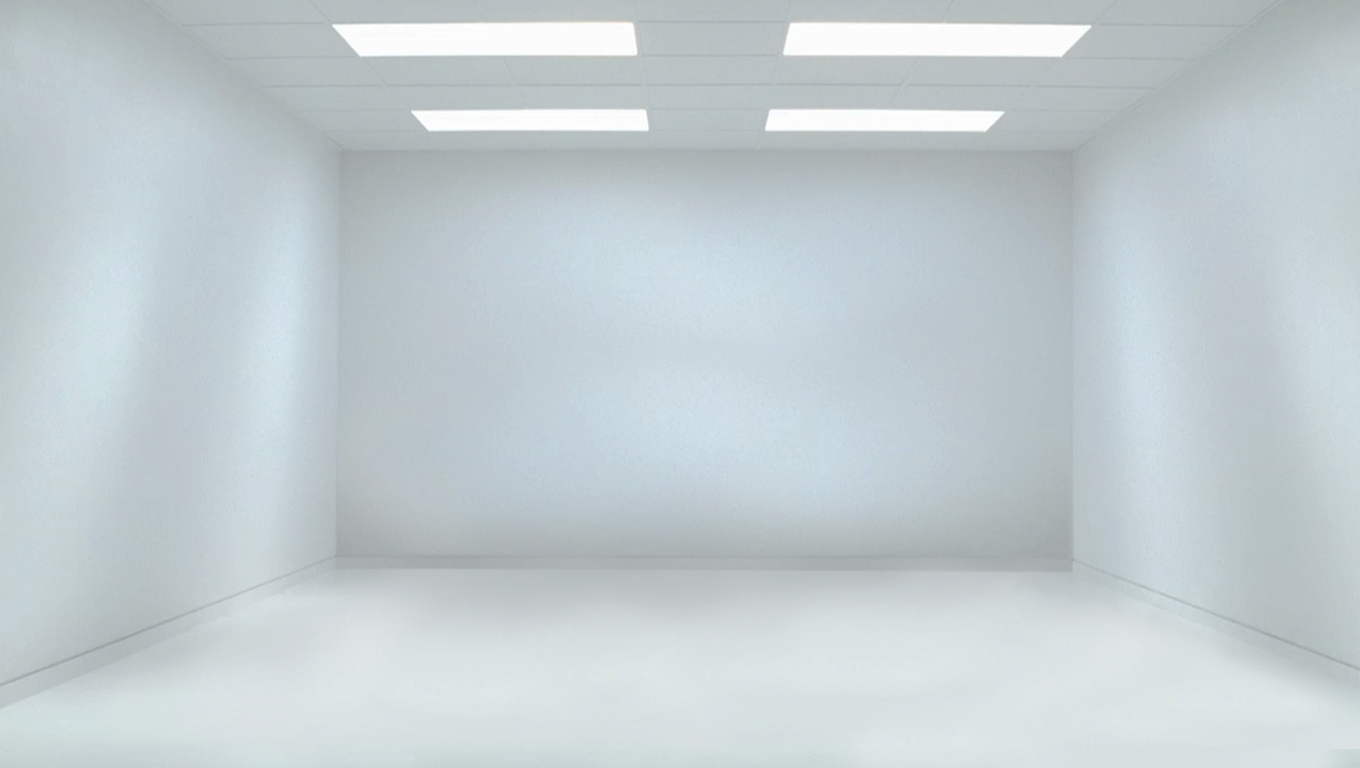
\includegraphics[width=1.175\paperwidth,height=1.05\paperheight]{./img/m1_praes_empty_10.jpg}%
}
\usetheme{default}
\author{user\thanks{user@mink}}
\date{15.4.2021}
\title{Interior Designer App: M1}
\subtitle{Problemanalyse}
\usetheme{Hannover}\usepackage{graphicx}\usepackage[overlay]{textpos}
\setbeamertemplate{bibliography item}{}
\setbeamertemplate{navigation symbols}{}
\definecolor{UBCblue}{HTML}{153a7a}\usecolortheme[named=UBCblue]{structure}
\usefonttheme{professionalfonts}
\setbeamerfont{note page}{family*=pplx,size=\footnotesize}
\definecolor{bgminted}{HTML}{eee9e9}
\definecolor{bluegray}{rgb}{0.54, 0.6, 0.8}
\definecolor{urlcolor}{HTML}{3399ff}
\definecolor{linkcolor}{HTML}{3399ff}
\definecolor{colorlinkscolor}{HTML}{3399ff}
\hypersetup{colorlinks=colorlinkscolor,linkcolor=linkcolor,urlcolor=urlcolor}
\setbeamertemplate{itemize items}[default]
\setbeamertemplate{enumerate items}[default]
\setbeamertemplate{items}[default]
\setbeamerfont*{title in sidebar}{shape=\scshape,size=\scriptsize}
\setbeamerfont*{author in sidebar}{family=\sfseries,size=\scriptsize}
\setbeamerfont*{section in sidebar}{family=\sfseries,size=\scriptsize}
\usetheme{Hannover}
\def\swidth{3.6cm}
\setbeamersize{sidebar width left=\swidth}
\setbeamertemplate{sidebar left}
{
{\usebeamerfont{title in sidebar}%
\vskip1.5em%
\usebeamercolor[fg]{title in sidebar}%
\insertshorttitle[width=\swidth,center,respectlinebreaks]\par%
\vskip1.25em%
}%
{%
\usebeamercolor[fg]{author in sidebar}%
\usebeamerfont{author in sidebar}%
\insertshortauthor[width=\swidth,center,respectlinebreaks]\par%
\vskip1.25em%
}%
\hbox to2cm{\hss\insertlogo\hss}
\vskip1.25em%
\hskip0.15cm\insertverticalnavigation{\swidth}%
\vfill
\hbox to2cm{\hskip0.25cm\usebeamerfont{subsection in
sidebar}\strut\usebeamercolor[fg]{subsection in
sidebar}\color{bluegray}\tiny\insertframenumber\hfill}%
\vskip6pt%
}%
\author[A.Oğuz, D.Pegler, S.Pum]{Asım Oğuz, Dominik Pegler, Sophia Pum}
\institute{Universität Wien, Fakultät für Informatik (SS2021)}
\hypersetup{
 pdfauthor={user},
 pdftitle={Interior Designer App: M1},
 pdfkeywords={},
 pdfsubject={},
 pdfcreator={Emacs 27.1 (Org mode 9.4.4)}, 
 pdflang={Germanb}}
\begin{document}

\maketitle

\section{Problembeschreibung}
\label{sec:org3e655d0}
\begin{frame}[label={sec:org0d9b9c3}]{\vspace{2.2cm}\begin{center}\MakeUppercase{\insertsection}\end{center}}
\end{frame}

\begin{frame}[label={sec:orgc03ec03}]{Interior Designer App}
\begin{block}{Problemstellung}
\begin{enumerate}
\item Welche Gestaltungsmöglichkeiten bieten Räume?
\item Wie können Möbel sinnvoll angeordnet werden?
\item Wie können auch Laien schnell zu Raumlösungen kommen und diese
visualisieren?
\end{enumerate}
\end{block}
\end{frame}
\begin{frame}[label={sec:org1e3a974}]{Interior Designer App}
\begin{block}{Lösungsansatz}
\begin{itemize}
\item Mobile App
\item User macht Bild von Raum
\item App vermisst Raum und Möbelstück
\item User platziert Möbelstück im Raum
\item App visualisiert Ergebnis
\end{itemize}
\end{block}
\end{frame}

\section{Literaturrecherche}
\label{sec:org68eb3a5}
\begin{frame}[label={sec:org7476519}]{\vspace{2.2cm}\begin{center}\MakeUppercase{\insertsection}\end{center}}
\end{frame}

\begin{frame}[label={sec:orgcfd74cd}]{Literatur}
\begin{block}{Schwerpunkt "Algorithmen und Augmented Reality"}
\begin{itemize}
\item \textcite{kanAutomatedInteriorDesign2017}
\item \textcite{sanduAugmentedRealityUses2018}
\item \textcite{moaresInterARInterior2020}
\end{itemize}
\end{block}
\end{frame}

\begin{frame}[label={sec:org5d5ff00}]{Literatur I}
\begin{block}{Automated Interior Design}
\begin{itemize}
\item \textcite{kanAutomatedInteriorDesign2017}
\item Algorithmus:
\begin{itemize}
\item befüllt Räume selbstständig mit Einrichtung
\item folgt Interior Design Guidelines zu Funktion, Ästhetik \& Ergonomie
\item Schneidet gut ab in Wahrnehmungsstudie
\end{itemize}
\end{itemize}
\end{block}
\end{frame}

\begin{frame}[label={sec:org8a7a6d1}]{Literatur II}
\begin{block}{Augmented Reality Uses in Interior Design}
\begin{itemize}
\item \textcite{sanduAugmentedRealityUses2018}
\item AR-unterstützte mobile Apps:
\begin{itemize}
\item OpenSource-Framework ArToolKit
\item Verbesserungsvorschläge zu aktuellen Implementierungen
\end{itemize}
\end{itemize}
\end{block}
\end{frame}

\begin{frame}[label={sec:org61e381b}]{Literatur III}
\begin{block}{Inter AR: Interior Decor App using Reality Technology}
\begin{itemize}
\item \textcite{moaresInterARInterior2020}
\item Arten von Augmented Reality
\begin{itemize}
\item marker-based vs. location-based vs. projection-based
\end{itemize}
\item Bericht Erstellung einer App mittels Google Cardboard SDK
\end{itemize}
\end{block}
\end{frame}

\section{Konkurrenzanalyse}
\label{sec:orga55a661}
\begin{frame}[label={sec:org3ba9ff0}]{\vspace{2.2cm}\begin{center}\MakeUppercase{\insertsection}\end{center}}
\end{frame}

\begin{frame}[label={sec:org803044f}]{Konkurrenzanalyse I}
\begin{block}{Houzz}
\begin{itemize}
\item \ldots{}
\item \ldots{}
\item \ldots{}
\end{itemize}
\end{block}
\end{frame}
\begin{frame}[label={sec:org2cc433d}]{Konkurrenzanalyse II}
\begin{block}{Ikea Place}
\begin{itemize}
\item \ldots{}
\item \ldots{}
\item \ldots{}
\end{itemize}
\end{block}
\end{frame}
\begin{frame}[label={sec:org4267e32}]{Konkurrenzanalyse III}
\begin{block}{Homestyler}
\begin{itemize}
\item \ldots{}
\item \ldots{}
\item \ldots{}
\end{itemize}
\end{block}
\end{frame}
\section{Nutzeranalyse}
\label{sec:orgbe94d21}
\begin{frame}[label={sec:orgf6276c9}]{\vspace{2.2cm}\begin{center}\MakeUppercase{\insertsection}\end{center}}
\end{frame}

\begin{frame}[label={sec:org6031bcc}]{Nutzeranalyse I}
\begin{block}{Aufgaben der Nutzer}
\begin{itemize}
\item Schnelles und unkompliziertes Skizzieren von Innenarchitekturen
\item Schnelle und unkomplizierte Visualisierung der gestalteten Innenarchitekturen
\item Die eigenen Vorstellungen anderen Personen einfach und anschaulich
zu kommunizieren
\end{itemize}
\end{block}
\end{frame}

\begin{frame}[label={sec:orgfc14395}]{Nutzeranalyse II}
\begin{block}{Ziele der Nutzer}
\begin{itemize}
\item Zeit- und Kostenersparnis, weil keine Beratung durch
Innenarchitekt*in nötig ist und die App an Ort und Stelle hilfreich
ist
\item Konkretere Vorstellungen zu entwickeln
\item Bessere und nachhaltigere Entscheidungen zu treffen
\end{itemize}
\end{block}
\end{frame}

\begin{frame}[label={sec:org408e3c9}]{Nutzeranalyse III}
\begin{block}{Potenzielle Probleme mit dem System}
\begin{itemize}
\item Die User fühlen sich von der App nicht angesprochen.
\item Die Funktionalitäten oder Auswahlmöglichkeiten sind zu
eingeschränkt, z.B. gibt es nur eine bestimmte Art von Möbeln oder
Objekten, die über die App darstellbar sind, oder es gibt technische
Limitationen mehre virtuelle Objekte gleichzeitig darzustellen.
\item Die User sehen den Nutzen nicht (wegen Art des Aufbaus der App nicht
klar ersichtlich)
\item App bringt keinen Zusatznutzen zu bereits vorhandenen Tools
\item User können Aufbau und Logik des Programms nicht nachvollziehen
\item Zu lange Ladezeiten (bei mobilen Apps noch wichtiger als bei Webapps!)
\item Freezing oder Absturz der App
\item Smartphone genügt den Anforderungen nicht
\end{itemize}
\end{block}
\end{frame}

\section{Personas}
\label{sec:org1c1d96e}
\begin{frame}[label={sec:orgefed52e}]{\vspace{2.2cm}\begin{center}\MakeUppercase{\insertsection}\end{center}}
\begin{center}
\vskip -12.5em 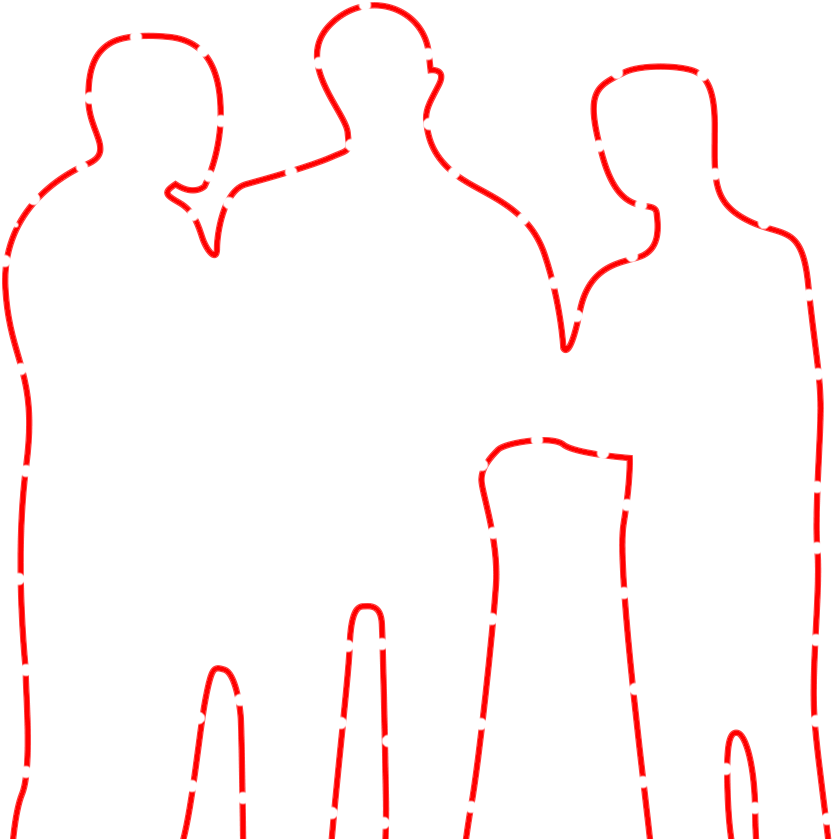
\includegraphics[height=140px]{./img/m1_praes_ol_persona3.png}
\end{center}
\end{frame}
\begin{frame}[label={sec:org1acf787}]{Personas I}
\begin{block}{Primäre Persona 1: Tobias Ebner}
\begin{center}

\includegraphics[width=90px]{./img/m1_persona_1_idealist.png}
\end{center}
\begin{itemize}
\item Typ: Idealist
\item Alter: 25
\item Beruf: Grafikdesigner
\end{itemize}
\end{block}
\end{frame}
\begin{frame}[label={sec:org64e88be}]{Personas II}
\begin{block}{Primäre Persona 2: Carina Winkler}
\begin{center}
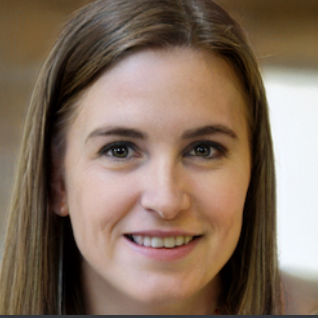
\includegraphics[width=90px]{./img/m1_persona_2_rational.png}
\end{center}
\begin{itemize}
\item Typ: Rational
\item Alter: 32
\item Beruf: Ärztin
\end{itemize}
\end{block}
\end{frame}
\begin{frame}[label={sec:org86a7a07}]{Personas III}
\begin{block}{Sekundäre Persona: Felix Schuster}
\begin{center}
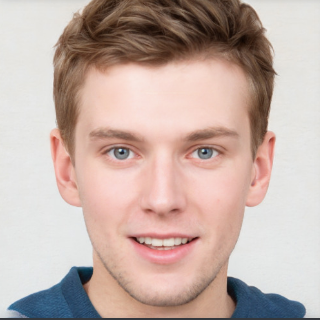
\includegraphics[width=90px]{./img/m1_persona_3_rational.png}
\end{center}
\begin{itemize}
\item Typ: Minimalist
\item Alter: 20
\item Beruf: Student
\end{itemize}
\end{block}
\end{frame}
\begin{frame}[label={sec:orgb44edc2}]{Personas IV}
\begin{block}{Negative Persona: Sabine Gruber}
\begin{center}
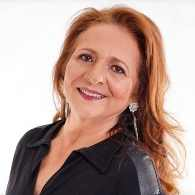
\includegraphics[width=90px]{./img/m1_persona_4_guardian.jpg}
\end{center}
\begin{itemize}
\item Typ: Guardian
\item Alter: 64
\item Beruf: Verkäuferin
\end{itemize}
\end{block}
\end{frame}
\section{Aufgabenanalyse}
\label{sec:orgdd4a9ed}
\begin{frame}[label={sec:orgcfaa784}]{\vspace{2.2cm}\begin{center}\MakeUppercase{\insertsection}\end{center}}
\end{frame}
\begin{frame}[label={sec:orgb687b12}]{Aufgabeanalyse}
\begin{itemize}
\item \ldots{}
\item \ldots{}
\item \ldots{}
\end{itemize}
\end{frame}
\section{Projektmanagement}
\label{sec:org15d2bc2}
\begin{frame}[label={sec:orgdc3238f}]{\vspace{2.2cm}\begin{center}\MakeUppercase{\insertsection}\end{center}}
\end{frame}

\begin{frame}[label={sec:org663486f}]{Projektmanagement I}
\begin{block}{Abstimmung und Planung}
\begin{itemize}
\item Simple Github-Page mit
\begin{itemize}
\item TODOs
\item Terminen und Deadlines
\item Zuordnung der Aufgaben
\item Notizen
\item Updates zum Fortschritt
\end{itemize}
\end{itemize}
\end{block}
\end{frame}

\begin{frame}[label={sec:org999aaec}]{Projektmanagement II}
\begin{block}{Aufgabenverteilung}
\begin{itemize}
\item nach Interesse und Themenblöcken
\item kurzfristig
\item flexibel
\end{itemize}
\end{block}
\end{frame}
\begin{frame}[label={sec:org38ba874}]{Projektmanagement III}
\begin{block}{Ziele des Projekts}
\end{block}
\end{frame}
\begin{frame}[label={sec:orge874eb9}]{Projektmanagement IV}
\begin{block}{Nicht-Ziele des Projekts}
\end{block}
\end{frame}
\section*{Literatur}
\label{sec:orgdcdd548}
\begin{frame}[allowframebreaks]{Literatur}
\printbibliography[heading=none]
\end{frame}
\appendix
\end{document}
